\chapter{Open heavy-flavour production in pp collisions}

Open heavy-flavour hadrons, i.e. those in which the heavy quark quantum number is expressed, made of one charm or beauty quark and other lighter quarks (such as D-mesons and B-mesons), can only be produced in processes with a high momentum transfer, because of the large mass of about 1.27 GeV and 4.18 GeV of the charm and beauty quarks, respectively. As such, they are created in the early stages of the collision, and their production cross-section in the partonic interaction can be evaluated perturbatively using QCD. The study of the production of open heavy-flavour hadrons in proton-proton collisions therefore provides an important test of the perturbative QCD framework and allows setting constraints on the models parameters. In addition, measurements of the production of open heavy-flavour hadrons in proton-proton collisions, where the production of a deconfined medium is not expected due to the low energy densities reached, are necessary ingredients for the study of heavy-ion collisions, where the properties of the QGP can be investigated. 

\section{Factorisation theorems}
The production of open heavy-flavour hadrons in proton-proton collisions can be described using the factorisation theorems~\cite{Collins:1989gx}, which allow separating the short-distance, perturbative behaviour from the long-distance, non-perturbative one. The total production cross-section can be expressed as:
\begin{equation*}
    \sigma_{\text{pp}} = \sum_\mathrm{a,b = g, q, \overline{q}} \int \de x_1 \de x_2 f_\mathrm{a/A}(x_1,\mu_F^2) f_\mathrm{b/B}(x_2,\mu_F^2) \hat{\sigma}_\mathrm{ab \rightarrow c} (x_1,x_2,\mu_F^2,\mu_R^2) D_\mathrm{c->H}(z,\mu_F^2) \quad ,
\end{equation*}
i.e. the convolution of; i. the Parton Distribution Functions (PDFs) $f_\mathrm{a/A}(x_1,\mu_F^2)$ and $f_\mathrm{b/B}(x_2,\mu_F^2)$, which describe the probability of finding a parton a in the proton A carrying a fraction of the proton momentum $x_1$, and a parton b in the proton B with a momentum fraction $x_2$, respectively; ii. the hard partonic scattering cross-section $\hat{\sigma}_\mathrm{ab \rightarrow c} (x_1,x_2,\mu_F^2,\mu_R^2)$, which describes the probability of producing the final state c from the collision of the partons a and b; and iii. the Fragmentation Functions (FFs) $D_\mathrm{c->H}(z,\mu_F^2)$, which describe the probability of a parton of type c fragmenting into a heavy-flavour hadron H with a momentum fraction $z$. While the PDFs and FFs are non-perturbative quantities, measured from data and then considered universal across different processes, the hard partonic scattering cross-section can be calculated perturbatively using QCD, but needs to be evaluated for each process. The factorisation theorems have been widely used to describe the production of open heavy-flavour hadrons in proton-proton collisions, and have proven to be successful in describing the data. Figure~\ref{fig:ppDmeson} shows the production cross-section of prompt and non-prompt $\mathrm{D^0}$-mesons in proton-proton collisions at $\sqrt{s} = 13$ TeV at midrapidity ($\lvert y\rvert<0.5$) as a function of the transverse momentum \pt measured by the ALICE experiment~\cite{ALICE:2021mgk}, compared to FONLL calculations~\cite{Cacciari:2001td}. The term \emph{prompt} refers to charm-hadrons produced directly in the hadronisation of a charm quark or the strong decay of a directly produced excited charm-hadron state, in contrast to \emph{feed-down} charm-hadrons, produced in the decay of a hadron containing a beauty quark. The FONLL predictions are in good agreement with the non-prompt $\mathrm{D^0}$-meson production cross-section, while the prompt contribution lies on the upper edge of the theoretical uncertainty band, albeit it is described within the uncertainties. This trend is also observed in the production of other open heavy-flavour hadrons and different experimental facilities, such as Tevatron, RHIC and LHC.

\begin{figure}
    \centering
    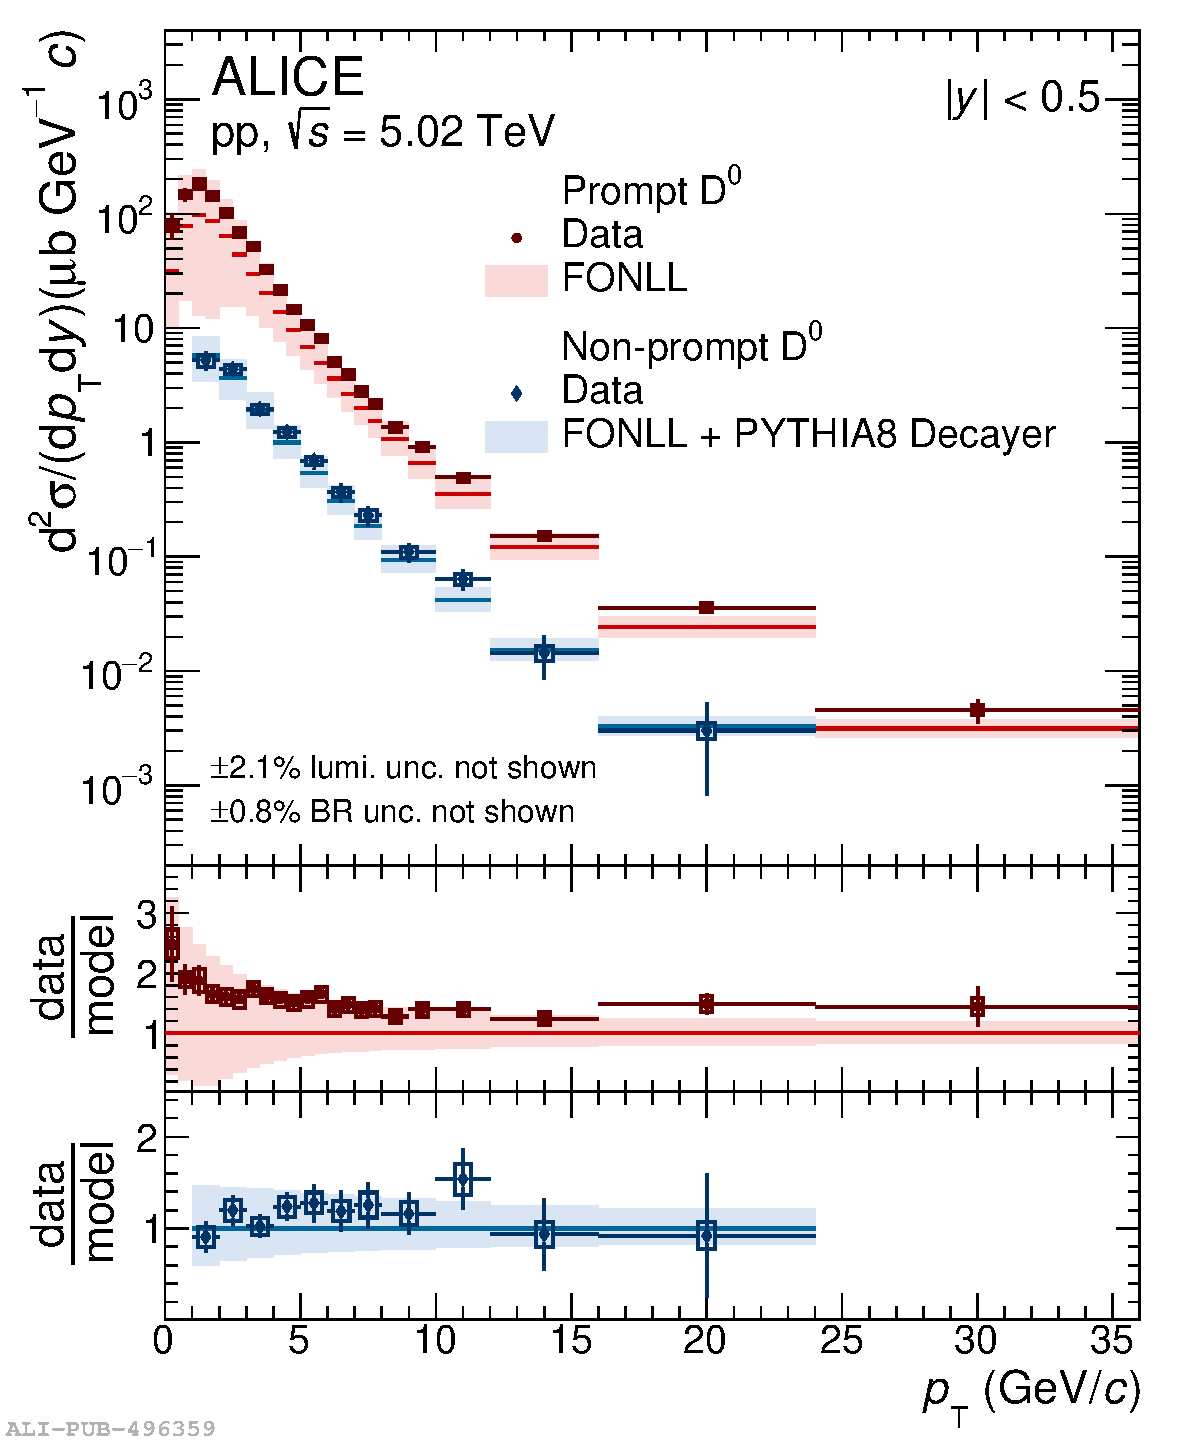
\includegraphics[width=0.48\linewidth]{Figures/Chapter 2/CrossSectionD0_Prompt_NonPrompt_pp5TeV_vsFONLL_Pythia8_BRnative_1.pdf}
    \caption{Caption}
    \label{fig:ppDmeson}
\end{figure}

\subsection{Parton Distribution Functions}


